\documentclass{article}
\usepackage[utf8]{inputenc}
\usepackage{url}
\usepackage[english]{babel}
\usepackage{amsmath}
\usepackage{amssymb}
\usepackage{nccmath}
\usepackage{graphicx}
\usepackage{subcaption}

\usepackage{tabularx}
\usepackage[ruled,vlined]{algorithm2e}
\usepackage{titling}
\newcommand{\PCAF}{(b)}
\newcommand{\PCAB}{(c)}
\newcommand{\NMFB}{(a)}
\newcommand{\FIGLABEL}[1]{Performance of #1 on test set}

% PCA Full Label
\newcommand{\PCAFL}{All Unbalanced PCA training data - 50 components}
% PCA Balanced Label
\newcommand{\PCABL}{Balanced subset of PCA training data - 50 components}
% NMF Balanced Label
\newcommand{\NMFBL}{Balanced subset of NMF training data - 70 components}

\newcommand{\subtitle}[1]{
  \posttitle{
    \par\end{center}
    \begin{center}\large#1\end{center}
    \vskip0.5em}
}
\usepackage{wrapfig}
\usepackage{float}

\usepackage{multicol}
\usepackage{geometry}
\geometry{legalpaper, margin=3cm}
\setlength{\columnsep}{1cm}

\usepackage[
backend=biber,
style=ieee
]{biblatex}

\addbibresource{bibliography.bib} %Imports bibliography file
\graphicspath{{Result Images/}}

\begin{document}

% - 10 to 15 pages up to a maximum of 25 pages
% ---------------------- Title Page-------
\title{Assignment 2 - Group: 25}
\subtitle{Tutors: Chen Chen, The Canh Dinh, Claire Hardgrove, Fengxiang He, Ella Qin, Thomas Selvaraj, Nguyen Hoang Tran, Kunze Wang, Zhiyi Wang, Henry Weld, and Yixuam Zhang}

\author{Group Members: \textbf{Alex Elias} (aeli0392, 5004077020)\and \textbf{Jordan Clark} (jcla0752, 500324901)\and Mariam Taoum}

\date{\today}


\maketitle

% ---------------------- Abstract -------
%- succinctly describe the rest of your report.
%- justified and in italics
%- one paragraph long
%- Include description of problem, significance, methods, results, and conclusion [3pt]
\section*{Abstract}
\emph{Statistical and Machine learning techniques are quickly becoming ubiquitous in the modern digital age, and there are many different techniques offered in literature that have various levels of performance on different problem domains. This makes it sometimes difficult to decide on which algorithms to use for a specific problem domain. This report provides a detailed comparison of different machine learning and data mining classification methods. By implementing different classification algorithms on the same classification problem, the algorithms can be compared by speed and accuracy on the problem domain. Various classification algorithms including Neural Networks, Logistic Regression, K - Nearest Neighbours (KNN), Gaussian Naive Bayes (GNB) and Linear and Quadratic Discriminant Analysis (QDA, LDA), were tested on the same chess positions classification problem. From these tests, we analysed the performance of the various algorithms and commented on their performance. From these results, we found that KNN performed best in terms of accuracy with the data set used in testing while Neural Networks performed best overall in terms of accuracy and run time. Future research can compare the algorithms on different data sets for more conclusive results. }
% -------------------------------------

% ------------------ Table of Contents--
\cleardoublepage
\tableofcontents
% -------------------------------------

% --------------- Introduction -------
%- should present the dataset that you chose, discuss its relevance in diverse applications, and give an overview of the methods you used.
%- What is the problem you intend to solve [3pt]?
%- Why is the problem important [2pt]?
\cleardoublepage
\begin{multicols}{2}
\section{Introduction}

In machine learning and data mining practices, several algorithms have been created to solve classification problems. However, since not all classification algorithms are the same, some are bound to be better suited for certain problems than others. In this report, we experiment with multiple algorithms to solve a classification problem and compare the performance and characteristics of the algorithms.
\\\\
While there are many commonly used classification algorithms, it is important to know which algorithm is best suited for the classification problem at hand, and classification problems in similar domains. By evaluating these different classification algorithms to solve the same classification problem, we can compare the performance of each algorithm and highlight the differences. We will also look at the run time complexity of each algorithm as this can have a large effect on the practicality of such methods.
\subsection{Problem Specification}
For this experiment, we used a Chess Positions dataset provided by kaggle \cite{kaggle}. This dataset contains 100000 chessboard images of chess positions, 80000 images in a training set, 20000 in a test set. Each chessboard image is made up of 400 by 400 pixels and contains between 5 and 15 pieces (2 of which are guaranteed to be kings). The dataset contains 28 board styles and 32 pieces styles. Using this dataset we trained three classes of algorithms: Neural Networks (Logistic Regression and Fully Connected Neural Network), Gaussian Models (GNB, LDA, QDA) and Nearest Neighbours (k = 5, 30 and 500), in an attempt to re-generate the original FEN description based on the board image. In this way, the chessboard image is classified as its FEN string \cite{FEN}. Since this problem is about classifying the board state, only the first section of the FEN string was used.
\\
\\
We will also show that this problem can be reduced to the classification of an individual square (1 of 64 per board) and its membership to one of 13 classes, black/white pieces (from 6 different categories) and blank squares. Due to the distribution of the generated dataset \cite{kaggle} the majority of the chessboard tiles split in this way are blank (there is no piece on the tile) $P\left(\mbox{blank tile}\right) \approx .8$. This creates an imbalanced dataset that we will address. While this problem adds some pre and post-processing, it reduces the (practically infinite) problem domain (all possible FEN strings = all possible chess board layouts) to just 13 classes.
%- TODO include??
%-More model hardware can be added as pre or post processing steps to encorperate relevant information that may be contained in other tiles within the same chess board (such as the board and piece styles)
\\\\
We will see that the problem can be reduced from a practically infinite problem, as the number of possible board states is infeasibly large to a classification to one of 13 classes with some additional information that can be leveraged. We will also define alternative evaluation metrics to assess models performance.
%- \textbf{(SIMPLIFICATION OF PROBLEM?)}

% ------------------------------------------------

% --------------- Previous Works ----------------
% -  explaining successful techniques utilised on the same or similar datasets and how they are different to yours
% - Describe previous relevant methods used in the literature [5pt] %- and how they are different to yours [5pt]

\section{Previous Works}
\subsection{Logistic regression and Artificial Neural Network}
Previous studies have been conducted to better compare various classification algorithms. For instance, Stephan Dreiseitl and Lucila Ohno-Machado conducted a study focusing on logistic regression and artificial neural network classification\cite{PWork}. The report was a methodology review of the two classification algorithms which illustrated how to build each algorithm, how to evaluate them, and what performance indices to report \cite{PWork}. In their meta-study, 72 studies that made both logistic and NN models where reviewed comparing the performance of artificial neural networks with logistic regression models \cite{PWork}. The results showed that there was a 5:2 ratio of cases in which its neural networks were not (statistically) significantly better then logistic regression \cite{PWork}.  
\\\\
This report has provided useful information on the methodology of both logistic regression and artificial neural network classification. Our research will go further to implement these algorithms and test them on this chess data set to compare their performance in practice. We will go further to also test K - Nearest Neighbours (KNN) Gaussian Naive Bayes and Linear Discriminant Analysis(LDA) algorithms with the same comparison metrics, and attempt to explain performance shortfalls / gains made by these other methods. We are also contributing a significantly different domain from this study, which was restricted to biomedical data \cite{PWork}.

\subsection{Classification for Imbalanced Datasets}
While imbalanced datasets appear frequently in real-world classification problems, they have the potential to negatively affect the performance of models\cite{PWork2}. Vaishali Ganganwar outlined some solutions to improve classification performance on unbalanced datasets \cite{PWork2}.
In classifying data with an unbalanced dataset, it is found that common classification evaluation techniques tend to be biased towards the majority class (\cite{BABoost}, \cite{PWork2}).
There are numerous ways to counter this, most relying on some sort of re-weighting of the importance of different observations as a function of its class\cite{PWork2}.
The BABoost method\cite{BABoost} adapts the AdaBoosts \cite{ADABoost} method of increasing the importance of misclassified and boundary cases to the unbalanced problem domain\cite{BABoost}.
Both methods provide improvements to classification algorithms performance by importance reweighting and BABoost improves the performance specifically on unbalanced datasets.
\\\\
These works have provided useful insights for dealing with imbalanced datasets which are useful to know since imbalanced datasets affect the accuracy of classification algorithms. Knowing this information will allow us to better handle the imbalanced dataset for our chessboard classification. While it is important to understand the effects of an unbalanced dataset on classification algorithms, our research differs from these findings in that we are provided metrics on the imbalanced dataset. That is we know the distribution of each chess piece and the likelihood of it occurring. 
We will also explore to what effect these problems of imbalanced datasets have when the size of the dataset is massive.
% ------------------------------------------------


% --------------- Methods -------------------
% - Explain the theory behind each of them and discuss your design choices. This part should at least include pre-processing approaches and machine learning techniques used.
% - Compare and analyse the theory behind the different techniques [9pts] (3 for each algorithm)
% - Provide reasoning for your choice of algorithms or your design [9pts] (3 for each algorithm)
% - Utilise pre-processing techniques. Describe and justify. [7pts]
\section{Methods}
For this experiment PCA, NMF, Neural Network, KNN, GNB, Linear and Quadratic Discriminant Analysis algorithms where chosen to evaluate and compare different supervised learning techniques. In order to have the background needed to discuss and contrast algorithms performance, we must understand how the algorithms work at at least a basic level. We will first discuss the pre-processing techniques used in this experiment and explain the reasoning behind using these techniques. Then we will describe the theory behind each classification used and discuss the differences and similarities of these models from a technical viewpoint. We will then describe the evaluation methods used for comparing the classification algorithms. 

\subsection{Pre-Processing}
\subsubsection{Principal Component Analysis (PCA)}
\textbf Principle \textbf Component \textbf Analysis (PCA) was originally built from principal axis theorem and proposed by  Karl Pearson in 1901\cite{PCA}. 
\\\\
The algorithm goes as follows:\\
Suppose you have a matrix $\mathbf X \in \mathbb{R}^{n, d}$ that represents your $n$ observations of $d$ features (that is your \emph{dataset}).
PCA takes an estimate of the variance-covariance matrix $\mathbf \Sigma$

\begin{align*}
\mathbf \Sigma &= E\left[\left(\mathbf X - E\left[\mathbf X\right]\right) \left(\mathbf X - E\left[\mathbf X\right]\right)\right]\\
&\approx {1 \over n-1} \sum\limits_{i=1}^n \left(x_i - \overline{\mathbf X}\right)
\left(x_i - \overline{\mathbf X}\right)^T
\end{align*}
where $x_i$ denotes the $i$th \emph{column} of $\mathbf X$ and $\overline{\mathbf X} = {1 \over n}\sum\limits_{i=1}^n \mathbf X_i$ is the sample mean.\\
\\
The eigenvalues of this matrix are proportional to the explained variance of its corresponding component (eigenvector). By ordering the eigenvectors by the size of their eigenvalues, we can select exactly how much of the variation to include, and how many of the components to use. This leaves us with a linear transformation that rotates and stretches data in the domain such that the first axis explains more variation then all others, then the second, etc.\\
\\
Since our dataset is large, we employed methods by D. Ross et al \cite{IncrementalPCA} to allow online learning of the components and explained variances; avoiding the need for the entire dataset to  fit into memory. Practically, the resulting projection achieved is equivalent to the offline method described above.
%- \subsubsection{Singular Value Decomposition (SVD)}
%- \tixtbf SinguVD is a pre-processing technique to reduce a dataset by decomposing the data matrix X into three matrices.
%- \begin{ceqn}
%- \begin{align}
%- X = U \Sigma V^T
%- \end{align}
%- \end{ceqn}
%- From this decomposition, matrix U is a $m \times r$  column-orthonormal matrix where r is the rank of the matrix. Matrix $\Sigma$ is a $r \times r$ diagonal. While matrix V is a $n \times r$ column-orthonormal.

\subsubsection{Non-Negative Matrix Factorization (NMF)}
\textbf Non-Negative \textbf Matrix \textbf Factorization (NMF) is a class of dictionary learning that enforces (or maintains) non-negativeness of the dictionary and the representation vector. (the dictionary in this context is similar to the components in the case of PCA)
\\
\\
The aim of NMF (like PCA) is to project $X \in \mathcal X$ into some vector subspace $\mathcal R = \mathbb R^k$ in a way that preserves the variation in the data:
\begin{equation}
X = RD
\end{equation}
The dimensions of the matrices are as follows:
\begin{align*}
    X &\in \mathbb R_{\ge 0}^{n, d}
    &
    R &\in \mathbb R_{\ge 0}^{n, k}
    &
    D &\in \mathbb R_{\ge 0}^{k, d}
\end{align*}
\\\\
This differs from PCA in this way. The specifics of how it is trained are beyond the scope of this report. For more information, see \emph{Algorithms for Non-Negative Matrix Factorization}\cite{NMF}. These differences prevent the dictionary from containing massive positive and massive negative numbers that counteract each other, and tends to have the effect of learning human-recognisable features in a way that is hopefully more representative of the features that the model should be training for. This could give NMF an edge over PCA in explainability and model performance when using models such as logistic regression, KNN and Gaussian Naive Bayes.

\subsubsection{PCA vs. NMF}
We have tried models using PCA transformed and NMF transformed data for all algorithms. The motivation behind this being that the process of NMF captures the correlation between different features (pixels) and encodes to describe the joint relationship, representing more of an abstract feature then an individual pixel. This may reduce the work-load of any of the models that need to be optimized (neural network and logistic regression models) and will not hurt the performance of others that do their own transformations (LDA and QDA) as their transformation will just encorperate the inverse of the rotation the PCA did with the model that it would have done otherwise. (The estimated sigmas will be closer to identity matrices). In addition to this, the dimensionality of the data can be reduced by about 5x, improving the speed (in the case of KNN) by up to 20 times (especially if the KNN is unoptimized).

\subsection{Classification Algorithms}
\subsubsection{Fully Connected Neural Network}
The Fully Connected Neural Network we trained is a supervised learning technique in which a model
$f : \mathcal X \mapsto \mathcal Y$ is trained with data
$\left(X,\,Y\right) \in \left(\mathcal X, \mathcal Y\right)$

The model structure is composed of layers, $l: \mathcal I \mapsto \mathcal O$ which hold the mathematical structure:

\begin{align*}
l_{W, b}\left(I\right) = O = I W + b
\end{align*}


Many of these layers are aggregated, the output of one becoming the input of the next.
As this would only allow linear models (the combination of many linear transformations) between layers a non linear activation function is used\footnote{Both preprocessing methods (PCA and NMF) are linear transformations on the data, and so could be thought of as pre-trained NN layers without an activation function. The advantage to using the pre-processing technique to pre-train and fix this layer is the convexity of the problem (and in the case of PCA the closed-form solution). The methods and implementations are also more mature.}. (examples include the sigmoid function\cite{sigmoid}, relu function\cite{ReLU} and leaky-relu function\cite{lReLU}).\\
\\
The data are fed as the input to the first layer, and the model is structured to have the final layers output in the same domain as the class labels (or the transformed class labels).\\
\\
The parameters for this model include all weights and biases (values for $W_l and b_l$) for all models.
These are trained using the SGD \cite{SGD} algorithm allowing arbritrarily complex models (that are differentiable).
This method simply treats the training data and labels as constants, leaving the loss function (which encorperates the model output) as a function only of the model parameters. Framed in this point of view, the derivative with respect to each parameter in the model is found, and a new value for the parameter is estimated $W_l_,_i^{t+1} \leftarrow W_l_,_i^t + \eta{\delta\over\delta W_l_,_i^t}\mbox{LOSS}$ where $\eta$ is the learning rate. Variants on this (stochastic, batch and mini-batch gradient descent) treat only parts of the training set as constant at a time, while the others are 0. (or non-existant) thus allowing the model to be trained on massive amounts of data with practical amounts of memory\cite{SBM-GD}. 

For our implementation we used mini-batch gradient descent with a neural network with 2 hidden layers of size 50 and 30.

\subsubsection{K - Nearest Neighbours (KNN)}
KNN is a classification algorithm in which observations are assumed to be the same as observations around it and therefor labeled as the same. In this method, a distance matrix is used to calculate the distance between records and a value $k$ is assigned as the number of neighbours to be evaluated\cite{KNN}. In classifying an unknown observation, the distance between the unknown observation (to be labelled) and the training records (known observations) is calculated. The $k$ training records closest to the unknown observation are aggregated and the most common label in the aggregation becomes the classification for that class.
\\\\
The accuracy of this method is affected by the choice of $k$. If $k$ is too large, points from other classes my be included effecting the majority class in the $k$ observations. Additionally, if $k$ is too small, the uncommon occurrence of another class may strongly effect the classification. Another concern about this algorithm is the scale of attributes. Attributes should be scaled before using KNN to prevent an attribute from dominating the distance matrix. This is a big issue that can arise with this method are attributes with different scales.

\subsubsection{Linear and Quadratic\footnote{QDA was not taught in this course and is the extra model we used} Discriminant Analysis(\{L,Q\}DA)}
Linear/Quadratic Discriminant Analysis are classification algorithms that focus on a distribution moddeling approach for classification.
The training dataset is fit to a mixture of gaussian distributions, with, in the case of Linear discriminant analysis common variance-covariance matrices.
Predictions are then made with the 
Using this information, the LDA model then makes predictions by calculating the probability that a new set of inputs belongs to each class, and decides the class that has the highest probability density at the new datapoints location.
The linear discriminant analysis is called so due to the decision boundary being linear.
With quadratic discriminant analysis the decision boundaries are quadratic conic sections due to the orientation of gaussians covariance matrices ability to have offset angles relative to one another.

\end{multicols}

\begin{figure}[h]
\begin{subfigure}{0.5\textwidth}
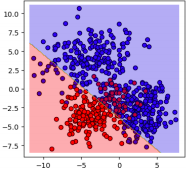
\includegraphics[\textwidth, height=5cm]{LDA.png} 
\centering
\caption{LDA}
\label{fig:subim1}
\end{subfigure}
\begin{subfigure}{0.5\textwidth}
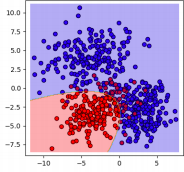
\includegraphics[\textwidth, height=5cm]{QDA.png}
\caption{QDA}
\label{fig:subim2}
\end{subfigure}

\caption{Experiments with multi-modal data: (a) LDA, (b) QDA}
\label{fig:LDA/QDA}

\end{figure}
\begin{multicols}{2}


LDA creates a linear decision boundary while QDA can create conic sections (including the linear case). From this, QDA can perform better on classification problems that do not have a clear linear boundary between classifications as seen in figure \ref{fig:LDA/QDA}. 

\subsubsection{Comparing Methods}
Neural Network and LDA models are similar in the fact that both models are supervised learning approaches, and both output conditional probability distributions. However, LDA assumes that each class of data follows a Gaussian distribution, with either shared or its own covariance matrix.
KNN is different in that the algorithm uses the data directly, without building a model for classification and heavily depends on the choice of $k$ and distance metric \cite{PWork}. 

\subsection{Evaluation Methods}
Classification algorithms are best evaluated in terms of accuracy, precision, recall, run time and with the use of a confusion matrix. Accuracy is the ratio of correct prediction compared to the total number of predictions. 

\begin{align*}
\mbox{Accuracy} = \frac{\mbox{Number of Correct Predictions}}{\mbox{Total number of Predictions}}
\end{align*}
Accuracy is not a good metric to use on datasets that are as imbalanced as the chess dataset, as a model that simply predicts the most frequent class will get a high score (in our case, a model that always predicts an empty square will get an accuracy of about 80\%). Other methods defined below address this\\

Precision measures the ration of correct positive results compared to the total number of predicted positive results.

\begin{align*}
\mbox{Precision} = \frac{\mbox{True Positives}}{\mbox{True Positives + False Positive}}
\end{align*}

Recall measures the ration of correct positive results competed to the total number of predictions that should be positive.   

\begin{align*}
\mbox{Recall} = \frac{\mbox{True Positives}}{\mbox{True Positives + False Negative}}
\end{align*}

As we are dealing with more then two classes (there is more then one type of false positive - true was B but guessed A vs true was C but guessed A) and more then one type of false negative (true was A but guessed B vs true was A but guessed C) we will include a weighted accuracy. This is the sum of all accuracy scores (as if the classes are only A and not A, B and not B etc) weighted by the proportion of observations that had that class. In general
\begin{align*}
    \mbox{Precision of }c = {\mbox{Predicted } c \mbox{ correctly} \over \mbox{Prediction was } c}
\end{align*}
\begin{align*}
    \mbox{Recall of }c = {\mbox{Predicted } c \mbox{ correctly} \over \mbox{True class was } c}
\end{align*}
Run time measures the time efficiently of the algorithm and it reports the amount of time it takes to run the classification algorithm. Confusion Matrix describes the performance of the model reporting true positives, true negatives, false positives and false negatives. 
% ------------------------------------------------


% --------------- Experiment ---------------------
% - displays results and comparisons for the implemented algorithms. Include runtime, hardware and software specifications of the computer that you used for performance evaluations. You are then expected to include meaningful comments on the results of your experiments, and reflect on your design choices.
% - Describe experiments, comparison and evaluation. Expected to fine tune each algorithm and explain why one approach outperforms the other. [15pts]
% - Meaningful discussion of results and design choices [5pts]
% - Provide relevant or meaningful personal reflection [5pts]
\section{Experiment and Discussion}
\subsection{Tools and Hardware}
An original chessboard in the provided JPEGs once loaded contains 400x400 pixels with 3 channels of color. If each pixel took 1 byte (with an unsigned int, the minimum it could) and there were 80000 examples to learn from, this would amount to $400\times 400\times 3 \times 80000$ bytes $= 35.76$GB of training data - without overheads of datastructures. Once these are converted to 32bit floats (as is needed for multiple of these algorithms) the size would quadruple. Even with the quick loading described earlier this would be too large to manage in memory and even in run time. Thankfully, this specific problem set lends itself well to being simplified, as intuitively the classification runs on black/white and shape. Immediately, color can be eliminated - thus reducing the size by 3 times. In addition, the 400x400 (split into 50x50) is a crisp image that makes viewing easy, but is not necessary to determine which piece is present. Theoretically, the machine learning algorithms can have the same classification as people, and as long as it is still possible to differentiate between the pieces (the information is not lost) the boards can be downscaled further.
We landed on 160x160 (split into 20x20 tiles) of black and white boards, a total reduction to a theoretical minimum of 1.90GB; a reduction in size by 19 times. In practise, the data takes about 2.4GB on the hard drive with compression, but we are storing it in a way that it is quick to load rather then minimizing space.
\\
\\
To further improve the performance, the chessboard matrices were stored in hdf5 files (each of 1000 examples).
If we were to store the raw image data without compression, the improvements in speed due to the lack of decompression start comparing with the extra time taken to read the larger file from disk. We found that a minor compression level reduced the filesize considerabely (reducing the former) without increasing decompression overhead (reducing the prior). Further improving the situation was to run compression over the area of one chessboard tile (20x20x3 in teh case of colored images downscaled to 160x160) maximizing the compression gains while not needing to decompress more then the data that is actually needed at one time (the single tile on the chessboard). This allowed for one tile to be read without the need to decompress the entire chessboard.
\\\\
From here, we saved the dataset as a reduced version (to not have to run the same computation again and again - a common theme in our implementation) and continued to our preprocessing step.
\\
\\
The preprocessing followed a similar theme, the PCA was computed on the training set and the components matrix was saved as to prevent it from needing to be recalculated over and over again.
The images were also transformed into the n-component vectors and saved to disk for quick lookup when training other models. (Or re-running the jupyter notebook)
A general tool was created that allowed any function to act in this way. For more details see the source code in the notebook provided named 'PreProcessing.ipynb'.

%- “section displays results and comparisons for the implemented algorithms. Include runtime, hardware and software specifications of the computer that you used for performance evaluations. You are then expected to include meaningful comments on the results of your experiments, and reflect on your design choices.” This template should be used as a starting point for your report.
\subsection{Experiments}
\subsubsection{PCA}
Deciding the number of components to use is a well defined problem. As described in section 3.1.1, we can easily control the variance/dimensionality tradeoff. Figure \ref{fig:PCA_nonorm} shows this trade-off explicitly. The x axis denotes the number of components to include (dimensionality) and the y axis denotes the amount of variation captured by the reduction. Shown as black lines, 50 components explains 98\% of the variation, and adding a further 50 components (to double the dimensionality) adds a further 1\% of variance. It is for this reason that the bulk of our analysis was done with 50 components. \ref{fig:PCA_recon} confirms this, with very little loss of detail after 50 components. It is also a good litmus test (although not sufficient) to look at some examples of reconstructions with varying levels of reduction. Figure \ref{fig:PCA_recon} shows this, with columns showing reconstruction from (left) 10, 30, 50, 70, 100 components then the original image on the right column. This also confirms that sufficient detail to make out the images is contained in the first 50 components\footnote{From this image it appears that even fewer are needed, but this is only a tiny sample of the data. The 4th row shows the knight is very difficult to identify below 50 components, even if the others are clear.}.

\begin{figure}[H]
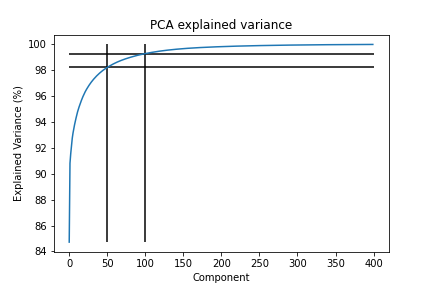
\includegraphics[width=\linewidth]{PCA_Explained_nonorm.png} 
\caption{PCA Explained Variance}
\label{fig:PCA_nonorm}
\end{figure}

%- PCA Reconstruction
\begin{figure}[H]
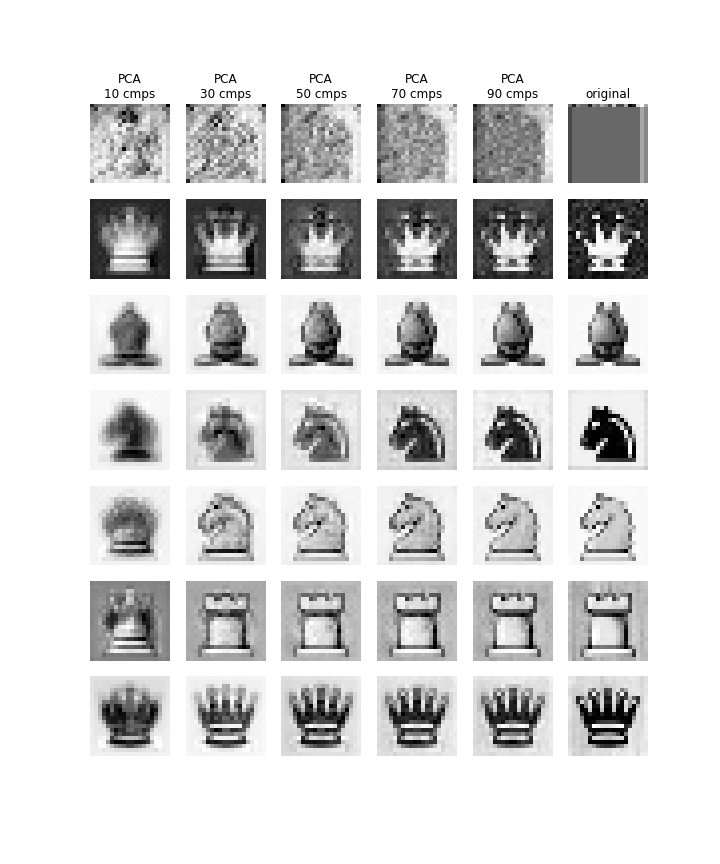
\includegraphics[width=\linewidth]{PCA_Reconstruction.png}
\caption{PCA Reconstruction}
\label{fig:PCA_recon}
\end{figure}

\subsubsection{NMF}
As discussed in the methods section of this report, we also evaluated performance on models with NMF reduction. Typically, NMF requires more components then PCA and we found 70 to be an appropriate number. Figure \ref{fig:NMF} illustrates the reconstruction results we managed with NMF. One notable result is the tendancy for noisy backgrounds to suddenly get 'ghosts' of pieces appear after being reconstructed through NMF (Figure \ref{fig:NMF} row 1 columns 3, 4 show a tile with some heavy grain, and the reconstruction has a ghostly rook). This sort of thing may be one reason why NMF models had marginally poorer performance.
%- NMF Reconstruction
\begin{figure}[H]
\centering
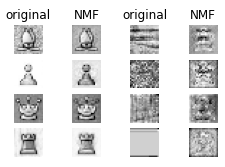
\includegraphics[width=\linewidth]{NMF_Reconstruction.png}
\caption{NMF Reconstruction}
\label{fig:NMF}
\end{figure}

\subsubsection{Background Removal}
Once PCA was trained, an attempt was made to remove the background of individual tiles, leveraging the information that every other tile is black and white. We devised an algorithm as follows:

\begin{algorithm}[H]
\SetAlgoNoLine
\KwResult{R has lost the information of the tile color}
R \in \mathbb R^{nxd}\leftarrow \mbox{image representations}\\
 B \leftarrow t \in R : \mbox{the color of t is Black}\\
 W \leftarrow t \in R : \mbox{the color of t is White}\\
 prop \in (0, 1)\\
 SD_B \leftarrow empty\ list\\
 SD_W \leftarrow empty\ list\\
 \For{i \in 1..d}{
    SD_B.append(sd(B[:, i]))\\
    SD_W.append(sd(W[:, i]))\\
 }\\
 \For{i \in 1..d}{
     \If{\mbox{rank of }SD_B[i] \le prop \times d} {
         B[:, i] \leftarrow 0\\
     }\\
     \\
     \If{\mbox{rank of }SD_W[i] \le prop \times d} {
         W[:, i] \leftarrow 0\\
     }\\
     continue\\
 }\\
 R \leftarrow \mbox{ recombine }B\mbox{ and }W\\
 \caption{Algorithm for tile color removal}
\end{algorithm}
This algorithm worked best on the PAC-transformed data, the results of which can be seen in figure \ref{fig:PCA_Background}. There are two columns of 5 (random) examples where the left of each column has the original image, and the right has the post-algorithm transformation.\\
We were very hopeful upon seeing the images that this would allow a second round of PCA, but upon closer inspection there are some issues. As shown in the first row, left column of figure \ref{fig:PCA_Background}, the black and white tiles have a fair amount of noise associated within colors, and this is made obvious in the selection algorithm on the top left, although as expected it has removed the bulk of the tile color.\\
The second problem is easiest to see on the first row on the right column, where the tile colors have been completely homogenised, but unfortunately as have some of the piece colors when they are on their own colored tile. (see pieces in the top right of the chessboard, the original clearly has different colored pieces while the selection algorithm transformed have been homogenized.)\\
It is for this reason that we decided not to continue with this method.


%- fine tuning 
\subsection{Evaluation}
For each type of model we looked at, we trained it on the full PCA transformed training set, the balanced subsample PCA transformed training set and the balanced bsample NMF training set. We also tried 3 different values of $k$ for KNN to attempt to discern between them. Figures \ref{fig:GNB} ,\ref{fig:LDA}, \ref{fig:QDA}, \ref{fig:5NN}, \ref{fig:30NN} and \ref{fig:500NN} show these results.
\\\\
% ----------- GNB, LDA, QDA ------------------
\subsection{Gaussian Models}
Figure \ref{fig:GNB} shows the model performance of the Gaussian Naive Bayes model, trained on the full PCA-transformed dataset \PCAF, trained on a balanced subsample of the PCA-transformed dataset \PCAB and trained on a balanced subsample of the NMF-transformed dataset \NMFB.
This is about aligned with our expectations, as even though GNB is unable to model correlation between features, the linear transformations of the NMF and GNB mean that no correlation on the transformed space could (and does) correspond to correlation on the original features.
One notable result here is that GNB has done much better on the full PCA dataset then on the balanced PCA dataset, indicating that the estimated distribution was much closer when given access to the extra data. This is also aligned with our expectations as more data in this instance will only bring the mean and sds contained within the model closer to their theoretical values for this datasets distribution.
Table \ref{tab:times} illustrates that this model trains extremely quickly, even on the full PCA dataset (of 5120000 observations) trained in only 0.41 seconds. This makes it a very powerful tool for getting a rudimentary feel if accuracy is to be sacrificed for speed. Further more, it was also among the fastest to predict in all categories.
\\\\
Figure \ref{fig:LDA} and Figure \ref{fig:QDA} show the model performance of the Linear Discriminant Analysis and Quadratic Discriminant Analysis respectively, trained on the full PCA-transformed dataset \PCAF, trained on a balanced subsample of the PCA-transformed dataset \PCAB and trained on a balanced subsample of the NMF-transformed dataset \NMFB. 
\\\\
Of the models tested in the experiment, these three models preformed the worse in terms of accuracy as seen in Table \ref{tab:performance}. This makes sense given that these models assume a Gaussian Distribution and - an assumption that seems to let these methods down. There are some interesting results here nonetheless: LDA has frequently predicted the blank tile more frequently then it appeared, as shown in figures \ref{fig:LDA} \NMFB, \PCAB and \PCAF. This contrasts with QDA (Figure \ref{fig:QDA}) which had the inverse problem - routinely predicting other classes when the true class was the empty tile, again on all models (Figures \ref{fig:LDA} \NMFB, \PCAF and \PCAB). Also interesting, is the LDA model trained on NMF-transformed data has some structure to its misclassifications; routinely correctly identifying either the piece color or the piece type (while not both at the same time). This is shown in Figure \ref{fig:LDA}\NMFB, by the square at the top left and bottom right (correctly guessing the color) and the diagonal lines offset from the main diagonal (correctly identifying the piece but not the color).
\\\\
The area where these models shine is in train and evaluation time. Table \ref{tab:times} shows that the GNB, LDA and QDA all trained among the fastest, rivaled only by the nearest neighbour models (which only copies the data). The story is similar in prediction time, but this time it is rivald by NN and LR, and balanced KNN models (their dataset search range is smaller).
\\\\
Overall these gaussian models do an excellent job taking the gaussian assumption into account. The reality is that the distribution of the pieces is far from gaussian (perhaps multimodal with different tile colors, board and piece styles)
% ------------ LR, NN ------------------------
\subsection{Neural Network and Logistic Regression}
Figure \ref{fig:LR} shows the model performance of the Logistic Regression model, trained on the full PCA-transformed dataset \PCAF, trained on a balanced subsample of the PCA-transformed dataset \PCAB and trained on a balanced subsample of the NMF-transformed dataset \NMFB. 
\\\\
This model resulted in high accuracy of .99 in both precision and recall on the full PCA-transformed dataset and NMF-transformed dataset and seen in Figure \ref{tab:performance}.
Additionally, the model had the fastest testing time on the full PCA-transformed dataset with only 599.39 seconds seen in Table \ref{tab:times}. It is important to note however that this model lacked in performance in terms of precision and recall in when it came to the balanced subsample of the PCA-transformed dataset. 
\\\\\
Figure \ref{fig:NN} shows the model performance of the Neural Network model trained on the full PCA-transformed dataset \PCAF, trained on a balanced subsample of the PCA-transformed dataset \PCAB and trained on a balanced subsample of the NMF-transformed dataset \NMFB. 
For examining the results of this model it is important to remember that the Neural Network model builds off the Logistic Regression model. This is seen from the Precision and Recall reported in Table \ref{tab:performance} which shows that the Neural Network model betters these performance metric, reporting near perfect accuracy. However, this increase in performance comes at a cost of training time as the Neural Network models takes significantly longer to train across all data sets. This is because iterative process of the gradient descent algorithm needed in the training process for the Neural Network. The model is also much more complex, with many more weights to train then in logistic regression. With smaller datasets, this can be a problem as the high complexity allows the model to 'memorize' the training dataset and the genralazation error skyrockets. As demonstrated in figure \ref{fig:NN}, this dataset has sufficient observations to render this a non-issue.
\\\\
Although the neural network had a long training time due to its necessity for gradient descent, its prediction time is very quick, making this model a good option if you have to train the model only once then use it many times.
% ------------- KNN --------------------------
\subsection{K Nearest Neighbours}
Finally, we have the K-Nearest Neighbours models in figures \ref{fig:5NN}, \ref{fig:30NN} and \ref{fig:500NN}. All around K-nearest neighbours performed impeccably getting precision and recall of 1 and 1 (IE all correct in the case of 5NN trained on the full unbalanced PCA-transformed training set) figure \ref{fig:5NN}\PCAF to precision and recall of .99 and .99 respectively (in the case of 500 Nearest Neighbours in figure \ref{500NN}\NMFB).
These results were much better then we had anticipated, and actually caused us to do an audit of the code to ensure the results were actually measured on the training set, and the training set had not been leaked in to the test set (it was and they had not).
We hypothesise that the sheer amount of data for the relatively low number of \emph{true} variation in the pieces (there were 892 piece style / board style combinations) compared to the ${512000 \over 13} \approx 40000$ examples per category leaves us with an estimated ${\sim40000 \over 892} \approx 44$ pieces per category, piece style, board style combination. This means that when KNN is looking for neighbours, there should be approximately 22 other pieces that look identical on the same color of tile with the same label\footnote{While this is the expected value, it may vary by a lot due to the nature of random numbers. Looking at the SD of this random variable is something we would like to do in a future study}. This means that for $k < \sim 44$ the $k$-nearest neighbours algorithm is effectively acting as a lookup table with some noise tolerance. This explains wholley how the model does so well. With this in mind, it is unsurprising that the model that performs the best is the 5-nn (irrespective of which dataset it was trained on) followed by 30-nn followed by 500-nn, as the higher neighbours increases the probability that the size of the cluster the test observation belongs to is smaller then k, meaning it starts to encompass other clusters.
\\\\
The time performance of the KNN models was among the worst for prediction. This is due to the large computational overhead of computing distances. sklearn does a good job of optimizing the problem, but there is only so far as it can go. This could make this method of classification infeasable despite its outstanding performance for many applications.
\\\\
Another way of viewing this is that due to the size of the training data, the model has been able to capture the (relatively simple) distribution $P\left(Y, X\right)$ extremely well.
\\\\
To study these results further, we would like to examine the distance that the KNN classifier has to expand to for misclassified labels compared to the distance for correctly classified observations. Another examination we could do is to perform an $892\times 13\times 2 = 23192$-means clustering (either mixture model or k-means) to attempt to capture this information, and examine the cluster sizes.
% ------------------------------------------------


% --------------- Conclusion ----------------------
% -  sum up your results and provide suggestion for meaningful future work.
% - Meaningful conclusion based on results, Meaningful future work suggested [3pts]
\section{Conclusion}
From these experiments, we can see that on the bases of accuracy, precision and recall, NN and KNN with 5 and 30 neighbours performed almost perfectly on all data sets. However, KNN with K as 5 and 30 took the longest to predict on the Balance NMF and PCA Full data sets. Given that some classification problems are time-sensitive, we have concluded that NN has shown to be the best model and preforms at best on the Balanced PCA dataset since this model has the highest performance accuracy and fastest testing time.  
\\\\
While this study suggests that KNN performed the best in terms of accuracy, these results may be specific to the data set chosen for this study. To come to a more conclusive result, similar tests should be performed on a variety of classification data sets and their results should be compared to be able to make stronger conclusive results.
% ------------------------------------------------
\end{multicols}


\begin{figure*}
\centering
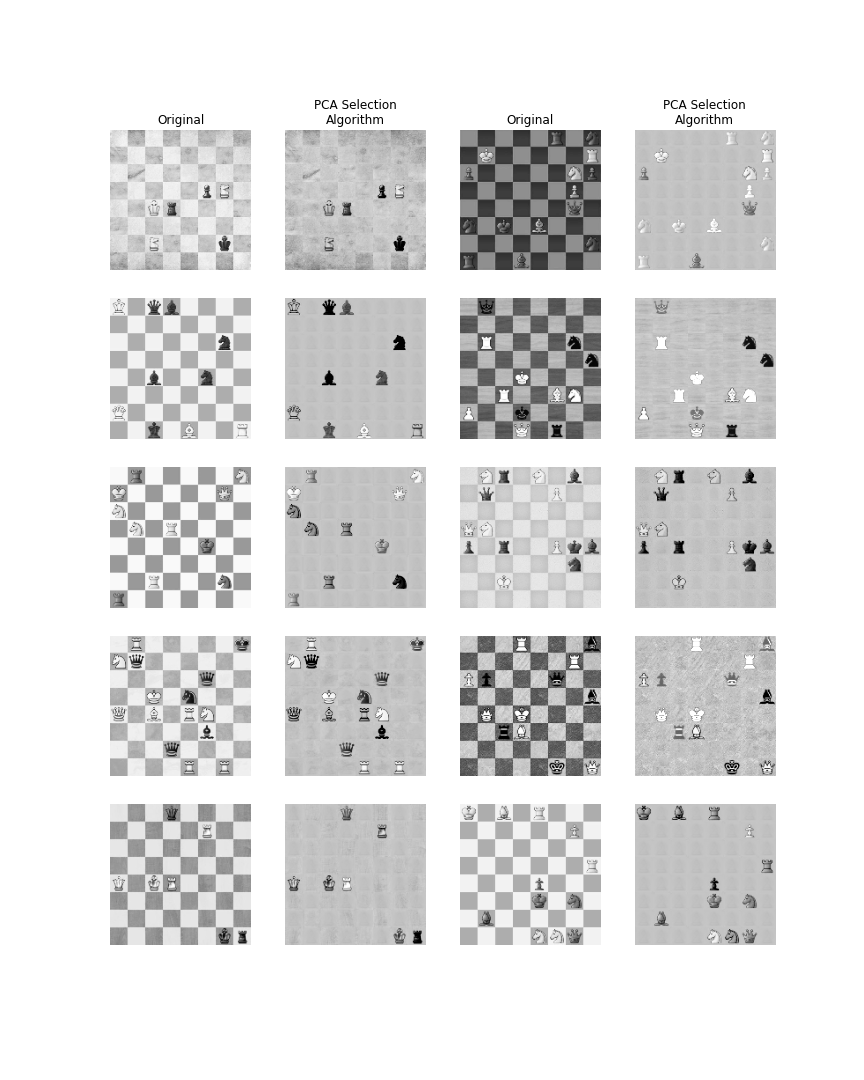
\includegraphics[scale=.38]{PCA_Background_remove_alg.png} 
\caption{PCA algorithm removing Background}
\label{fig:PCA_Background}
\end{figure*}

%------------------ Gaussian Naive Bayes
\begin{figure}[h]
\begin{subfigure}{0.33\textwidth}
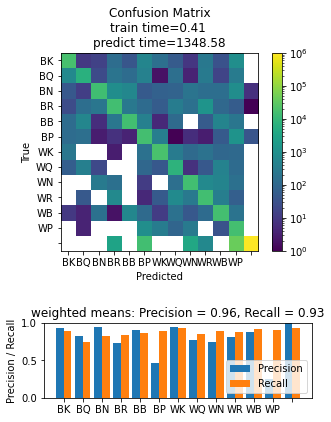
\includegraphics[width=0.9\linewidth]{GNB_B_NMF70c_160x160_evaluation.png} 
\caption{\NMFBL}
\end{subfigure}
\begin{subfigure}{0.33\textwidth}
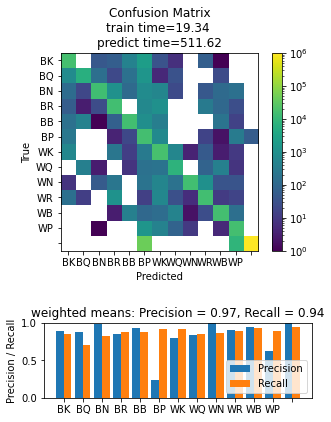
\includegraphics[width=0.9\linewidth]{GNB_PCA50c_160x160_evaluation.png}
\caption{\PCAFL}
\end{subfigure}
\begin{subfigure}{0.33\textwidth}
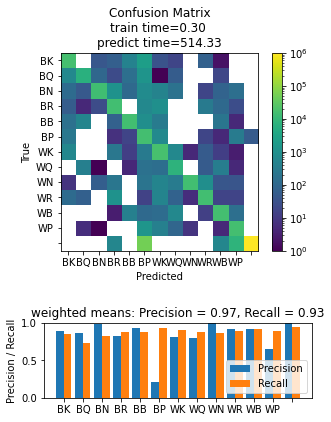
\includegraphics[width=0.9\linewidth]{GNB_B_PCA50c_160x160_evaluation.png} 
\caption{\PCABL}
\end{subfigure}
\caption{\FIGLABEL{Gaussian Naive Bayes}}
\label{fig:GNB}
\end{figure}

% ------------------- LDA ------------
\begin{figure}[h]
\begin{subfigure}{0.33\textwidth}
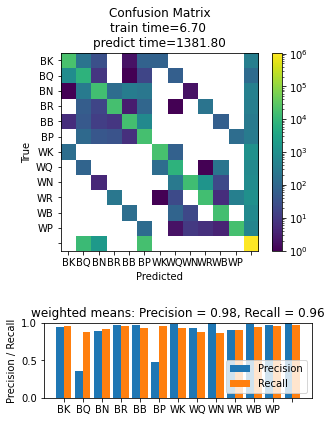
\includegraphics[width=0.9\linewidth]{LDA_B_NMF70c_160x160_evaluation.png} 
\caption{\NMFBL}
\end{subfigure}
\begin{subfigure}{0.33\textwidth}
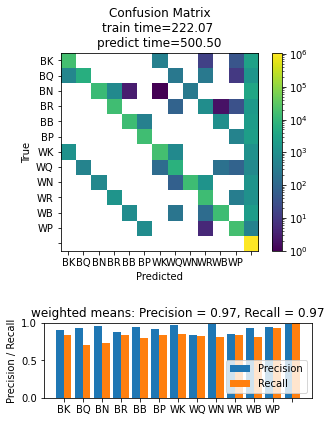
\includegraphics[width=0.9\linewidth]{LDA_PCA50c_160x160_evaluation.png}
\caption{\PCAFL}
\end{subfigure}
\begin{subfigure}{0.33\textwidth}
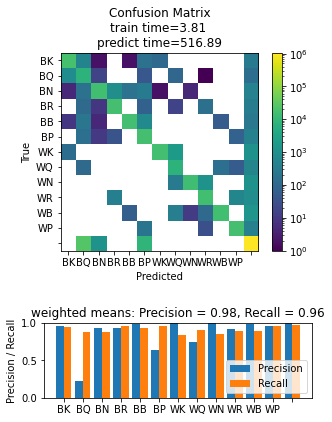
\includegraphics[width=0.9\linewidth]{LDA_B_PCA50c_160x160_evaluation.png} 
\caption{\PCABL}
\end{subfigure}
\caption{\FIGLABEL{Linear Discriminant Analysis}}
\label{fig:LDA}
\end{figure}


%----------------  Quadratic Discriminant Analysis
\begin{figure}[h]
\begin{subfigure}{0.33\textwidth}
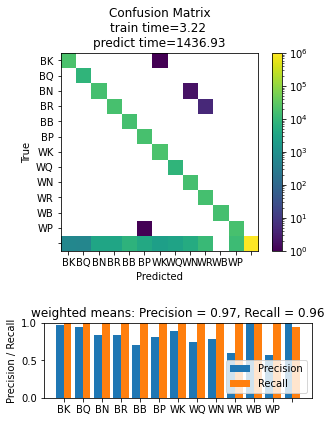
\includegraphics[width=0.9\linewidth]{QDA_B_NMF70c_160x160_evaluation.png} 
\caption{\NMFBL}
\label{fig:subim1}
\end{subfigure}
\begin{subfigure}{0.33\textwidth}
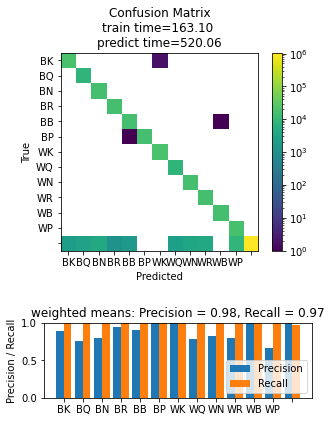
\includegraphics[width=0.9\linewidth]{QDA_PCA50c_160x160_evaluation.png}
\caption{\PCAFL}
\label{fig:subim2}
\end{subfigure}
\begin{subfigure}{0.33\textwidth}
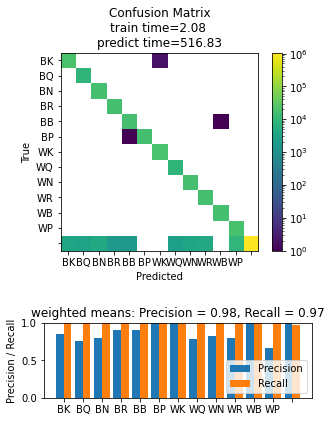
\includegraphics[width=0.9\linewidth]{QDA_B_PCA50c_160x160_evaluation.png} 
\caption{\PCABL}
\label{fig:subim3}
\end{subfigure}
\caption{\FIGLABEL{Quadratic Discriminant Analysis}}
\label{fig:QDA}
\end{figure}


% ------------------- Logistic Regression
\begin{figure}[h]
\begin{subfigure}{0.33\textwidth}
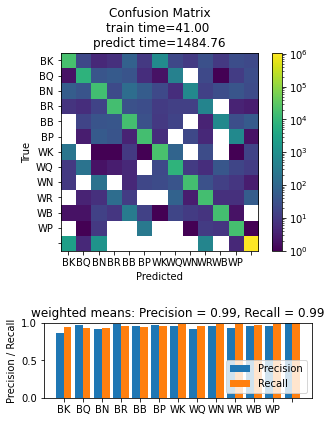
\includegraphics[width=0.9\linewidth]{LR_B_NMF70c_160x160_evaluation.png} 
\caption{\NMFBL}
\end{subfigure}
\begin{subfigure}{0.33\textwidth}
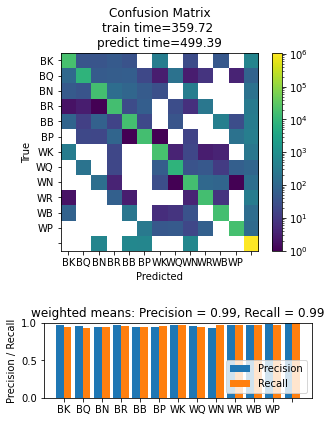
\includegraphics[width=0.9\linewidth]{LR_PCA50c_160x160_evaluation.png}
\caption{\PCAFL}
\end{subfigure}
\begin{subfigure}{0.33\textwidth}
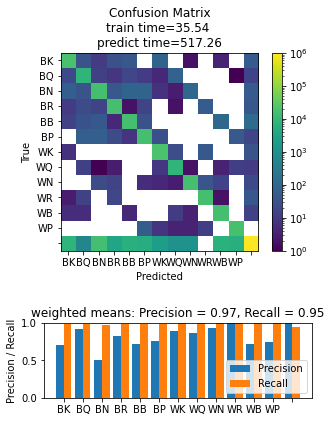
\includegraphics[width=0.9\linewidth]{LR_B_PCA50c_160x160_evaluation.png} 
\caption{\PCABL}
\end{subfigure}
\caption{\FIGLABEL{Logistic Regression}}
\label{fig:LR}
\end{figure}

%------------------- Neural Network
\begin{figure}[h]
\begin{subfigure}{0.33\textwidth}
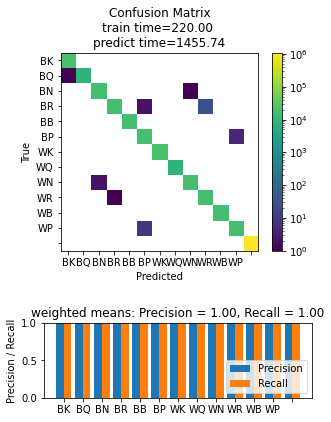
\includegraphics[width=0.9\linewidth]{NN_B_NMF70c_160x160_evaluation.png} 
\caption{\NMFBL}
\end{subfigure}
\begin{subfigure}{0.33\textwidth}
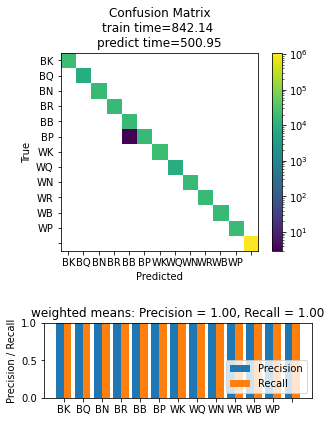
\includegraphics[width=0.9\linewidth]{NN_PCA50c_160x160_evaluation.png}
\caption{\PCAFL}
\end{subfigure}
\begin{subfigure}{0.33\textwidth}
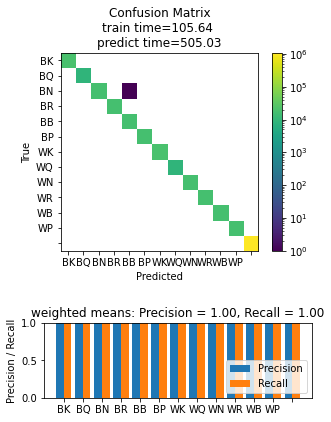
\includegraphics[width=0.9\linewidth]{NN_B_PCA50c_160x160_evaluation.png} 
\caption{\PCABL}
\end{subfigure}
\caption{\FIGLABEL{Neural Network}}
\label{fig:NN}
\end{figure}

%------------------- 5 KNN
\begin{figure}[h]
\begin{subfigure}{0.33\textwidth}
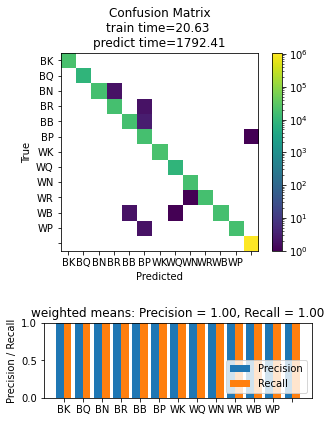
\includegraphics[width=0.9\linewidth]{5NN_B_NMF70c_160x160_evaluation.png} 
\caption{\NMFBL}
\end{subfigure}
\begin{subfigure}{0.33\textwidth}
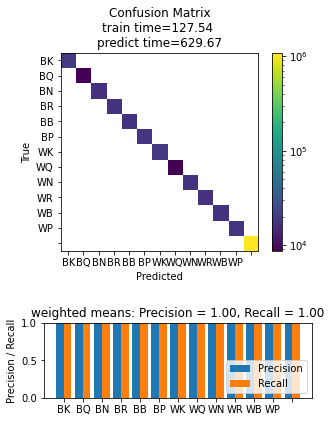
\includegraphics[width=0.9\linewidth]{5NN_PCA50c_160x160_evaluation.png}
\caption{\PCAFL}
\end{subfigure}
\begin{subfigure}{0.33\textwidth}
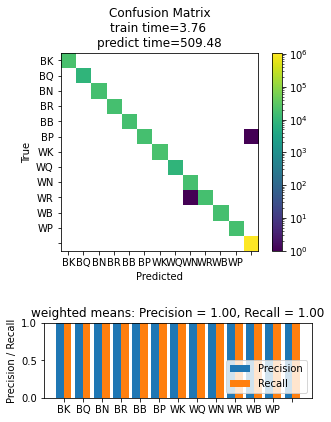
\includegraphics[width=0.9\linewidth]{5NN_B_PCA50c_160x160_evaluation.png} 
\caption{\PCABL}
\end{subfigure}
\caption{\FIGLABEL{5 Nearest Neighbours}}
\label{fig:5NN}
\end{figure}

%------------------- 30 KNN
\begin{figure}[h]
\begin{subfigure}{0.33\textwidth}
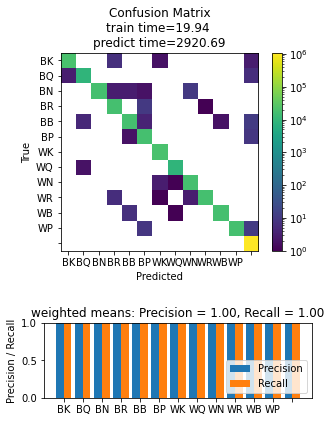
\includegraphics[width=0.9\linewidth]{30NN_B_NMF70c_160x160_evaluation.png} 
\caption{\NMFBL}
\end{subfigure}
\begin{subfigure}{0.33\textwidth}
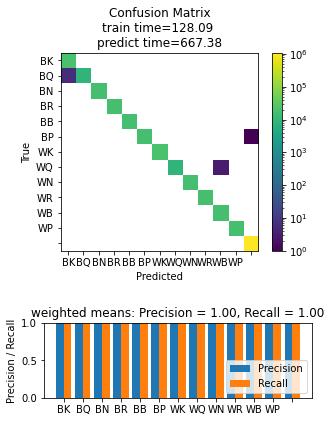
\includegraphics[width=0.9\linewidth]{30NN_PCA50c_160x160_evaluation.png}
\caption{\PCAFL}
\end{subfigure}
\begin{subfigure}{0.33\textwidth}
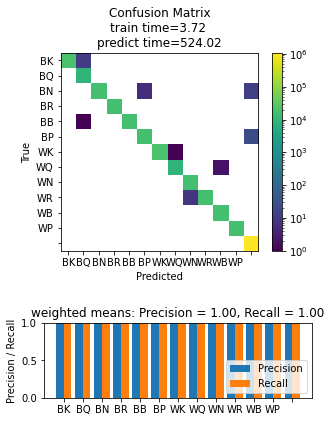
\includegraphics[width=0.9\linewidth]{30NN_B_PCA50c_160x160_evaluation.png} 
\caption{\PCABL}
\end{subfigure}
\caption{\FIGLABEL{30 Nearest Neighbours}}
\label{fig:30NN}
\end{figure}


%------------------- 500KNN
\begin{figure}[h]
\begin{subfigure}{0.33\textwidth}
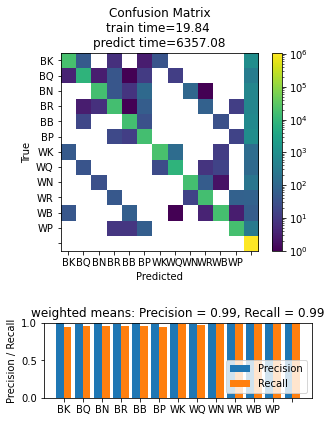
\includegraphics[width=0.9\linewidth]{500NN_B_NMF70c_160x160_evaluation.png} 
\caption{\NMFBL}
\end{subfigure}
\begin{subfigure}{0.33\textwidth}
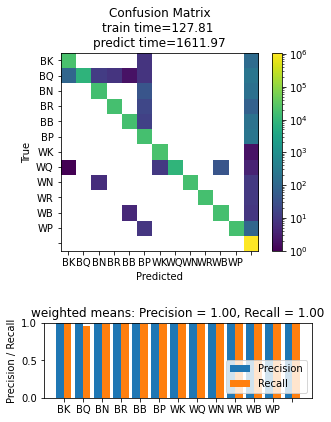
\includegraphics[width=0.9\linewidth]{500NN_PCA50c_160x160_evaluation.png}
\caption{\PCAFL}
\end{subfigure}
\begin{subfigure}{0.33\textwidth}
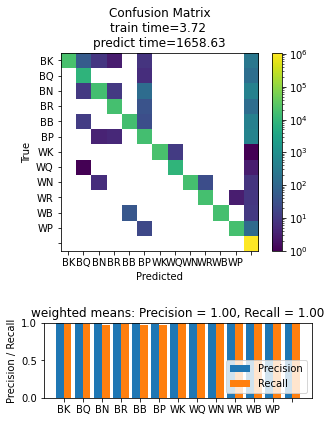
\includegraphics[width=0.9\linewidth]{500NN_B_PCA50c_160x160_evaluation.png} 
\caption{\PCABL}
\end{subfigure}
\caption{\FIGLABEL{500 Nearest Neighbours}}
\label{fig:500NN}
\end{figure}

% --------------------- Precision, Recall table ----------

\squeezetable
\begin{table}
\caption {\label{tab:performance} Weighted performance metrics} 
\begin{ruledtabular}
\begin{tabular}{llllllll}
 Model & \multicolumn{3}{c}{Precision} &  & \multicolumn{3}{c}{Recall}    \\ 
\cline{2-4} \cline{6-8} 
        & Balanced NMF   & PCA Full   &  Balanced PCA                                             &             
	&  Balanced NMF  & PCA Full   & Balanced PCA                                                 \\    \hline
 GNB   & 0.96   & 0.97 & 0.97  &         % done
       & 0.93   & 0.94 & 0.93 \\         % done
 LDA   & 0.98   & 0.97 & 0.98 &          % done
       & 0.96   & 0.97 & 0.96\\          % done
 QDA   & 0.97   & 0.98 & 0.98 &         % done
       & 0.96   & 0.97 & 0.97\\         % done
 LR & 0.99 & 0.99 & 0.97 &               % done
    & 0.99 & 0.99 & 0.95    \\           % done
 NN & \textbf{1.00}    & \textbf{1.00}   & \textbf{1.00}    &       % done
    & \textbf{1.00}   & \textbf{1.00}    & \textbf{1.00}    \\      % done
 5NN & \textbf{1.00}    & \textbf{1.00}    & \textbf{1.00}  &       % done
     & \textbf{1.00}  & \textbf{1.00}    & \textbf{1.00}    \\      % done
 30NN   & \textbf{1.00} & \textbf{1.00}    & \textbf{1.00}  &       % done
    & \textbf{1.00}   & \textbf{1.00}    & \textbf{1.00}    \\      % done
 500NN  & 0.99 & \textbf{1.00}    & \textbf{1.00}  &       % done
    & 0.99   & \textbf{1.00}   & \textbf{1.00} \\          % done

\end{tabular}
\end{ruledtabular}
\begin{tabbing}
\end{tabbing}
\end{table}

% --------------------- Train time table ----------

\squeezetable
\begin{table}
\caption {\label{tab:times} Run Time (seconds)}
\begin{ruledtabular}
\begin{tabular}{llllllll}
 Model & \multicolumn{3}{c}{Training - excluding transformation} &  & \multicolumn{3}{c}{Testing - including transformation}    \\ 
\cline{2-4} \cline{6-8} 
        & Balanced NMF   & PCA Full   &  Balanced PCA                                             &             
	&  Balanced NMF  & PCA Full   & Balanced PCA                                                 \\    \hline
 GNB   & \textbf{0.41}   & \textbf{19.34} & \textbf{0.30}  &
    & \textbf{1348.58}   & 511.62 & 514.33         \\ 
 LDA   & 6.70    & 222.07 & 3.81 &
    & 1381.80   & 500.50 & 516.89           \\
 QDA   & 3.22   & 163.10    & 2.08  &
    & 1436.93   & 520.06    & 516.83        \\
 LR & 41.00 & 359.72    & 35.54 &
    & 1484.76   & \textbf{499.39}    & 517.26    \\
 NN & 220.00    & 842.14    & 105.64    &
    & 1455.74   & 500.95    & \textbf{505.03}    \\
 5NN & 20.63    & 127.54    & 3.76  &
    & 1792.41   & 629.67    & 509.48    \\
 30NN   & 19.94 & 128.09    & 3.72  &
    & 2920.69   & 667.38    & 524.02    \\
 500NN  & 19.84 & 127.81    & 3.72  &
    & 6357.08   & 1611.97   & 1658.63 \\

\end{tabular}
\end{ruledtabular}
\begin{tabbing}
\end{tabbing}
\end{table}


% ------------------ References -------------------
\cleardoublepage
\printbibliography
% -------------------------------------------------


% ---------------- Appendix -----------------------
\cleardoublepage
\begin{appendix}
\section{Appendix}
\subsection{On running the provided source code}
To run the source code and predict a random subset of 500 examples of the training set, the following procedure is needed:
\begin{enumerate}
    \item ensure the libraries listed in the next section are installed properly, and are linked to the same python runtime that jupyter notebook uses.
    \item extract the provided 'submission.zip' to a folder, maintaining structure. There should be a subdirectory called .cache. This is important.
    \item copy the training data from the kaggle website \cite{kaggle} into a directory called dataset/test/. This directory should now have many images. For example, with the root directory being the root of the archive, the file /data/test/rrQb2k1-q3R3-PR6-8-8-K3r3-p7-n2N2N1.jpeg should exist.
    \item With the directory containing all the ipynb files as the root directory, start a jupyter notebook and launch the notebook named 'Run This Notebook.ipynb'
    \item run all cells in the notebook, and observe the output.
\end{enumerate}
\subsection{Required Libraries}
\begin{itemize}
    \item numpy = 1.19.0
    \item pandas = 1.1.1
    \item opencv-python = 4.2.0.34
    \item matplotlib = 3.2.2
    \item h5py = 2.10.0
    \item scikit-learn = 0.23.2
    \item torchvision = 0.8.1
\end{itemize}
\subsection{Additional notes}
The original group has 3 members, including Mariam Taoum however received 0 contribution from here since we where not able to contact her.

\end{appendix}
% -------------------------------------------------

\end{document}